\section{引言}\label{introduction}

\subsection{软件维护}

软件维护旨在发现和解决软件项目中的漏洞,并且管理重要功能模块的软件变更。作为软件工程中一项关键过程,软件维护需要显著的时间与经济支出。\cite{SOLEIMANINEYSIANI2020106344} 随着现代软件规模的不断增长,软件维护的困难程度也在不断攀升。软件变更分析是软件维护的关键难题之一,其聚焦于变更代码对存量代码的影响,希望通过分析变更代码与变更所影响的代码进行软件维护,从而避免对全量代码的分析,降低软件维护的成本。

\subsection{AOSP (Android Open Source Project)}

Android 由 “开放手机联盟” (Open Handset Alliance) 的开发者联盟开发,谷歌对其提供商业赞助。Android 是一种基于改良版本 Linux 内核与其他开源软件的移动端操作系统,其本质是基于 Linunx 的开放源代码软件栈,主要为触屏智能移动设备而设计\cite{PLATFORMARCHITECTURE}。Android 本身由两部分组成,一部分是大多数 Android 设备都预装的额外专有软件,其中包括谷歌 Chrome、数字发行平台谷歌 Play 和相关的谷歌 Play 服务开发平台,这些核心应用统称为谷歌移动服务 (GMS)。而另一部分则是遵守 Apache License 的免费开源软件,这一部分软件项目被统称为 AOSP,意为 “Android 开源项目”。

作为首个为移动端打造真正开放和完整的移动软件,Android 是全世界占有率最大的移动操作系统,同时也是一个适用于消费类产品的完整高品质操作系统,并且配有可自定义并移植到几乎所有设备的源代码,以及所有用户均可使用的公开文档。

\subsection{Android 软件栈架构简述}

Android 是一种基于 Linux 的开放源代码软件栈,为各类设备和机型而创建。Android 整体架构被划分为五层,分别是 Linux 内核层、硬件抽象层、Android Runtime 与 C/C++ Lib、Java API 框架以及系统应用层。Android 软件栈架构图可见图 \ref{fig:android-stack}。

\begin{itemize}
    \item Android 软件栈的最底层是 Linux 内核部分,其利用 Linux 内核中的进程与线程管理、内存管理、设备管理、文件管理等功能,为上层的 Android 程序开发提供有效的平台基础。由于 Android 软件堆栈中的 Linux 内核部分可以利用 Linux 内核执行底层功能,因此,Android 有能力进一步为更高层的应用提供对基础功能的再抽象能力。
    \item Android 软件栈的第二层是硬件抽象层 (Hardware Abstraction Layer) 。硬件抽象层负责再包装 Linux 内核层提供的硬件能力。HAL 包含多个库模块,其中每个模块都为特定类型的硬件组件实现一个界面,例如相机和蓝牙模块。当框架 API 要求访问设备硬件时,Android 系统将为该硬件组件加载库模块。
    \item Android 软件栈的第三层是 Android Runtime 和 C/C++ Lib。对于运行 Android Lolipop(API 级别 21)或更高版本的设备,每个应用都在其自己的进程中运行,并且有其自己的 Android Runtime 实例。ART 编写为通过执行 DEX 文件在低内存设备上运行多个虚拟机,DEX 文件是一种专为 Android 设计的字节码格式,经过优化,使用的内存很少。编译工具链将 Java 源代码编译为 DEX 字节码,使其可在 Android 平台上运行。
    \item Android 软件栈的第四层是 Java API Framework。该层建立在底层 Android Runtime 和 C/C++ Lib 之上,为 Android 应用开发者提供应用开发所需要的工具与框架。Java API Framework 作为开发者可以直接且完全访问的 Android 系统应用使用的框架 API,封装了整个 Android 操作系统的所有功能。
    \item Android 软件栈的第五层是系统应用层。该层与用户直接交互,用于装载 Android 系统内置以及用户所开发的应用软件。
\end{itemize}

\begin{figure}
    \centering
    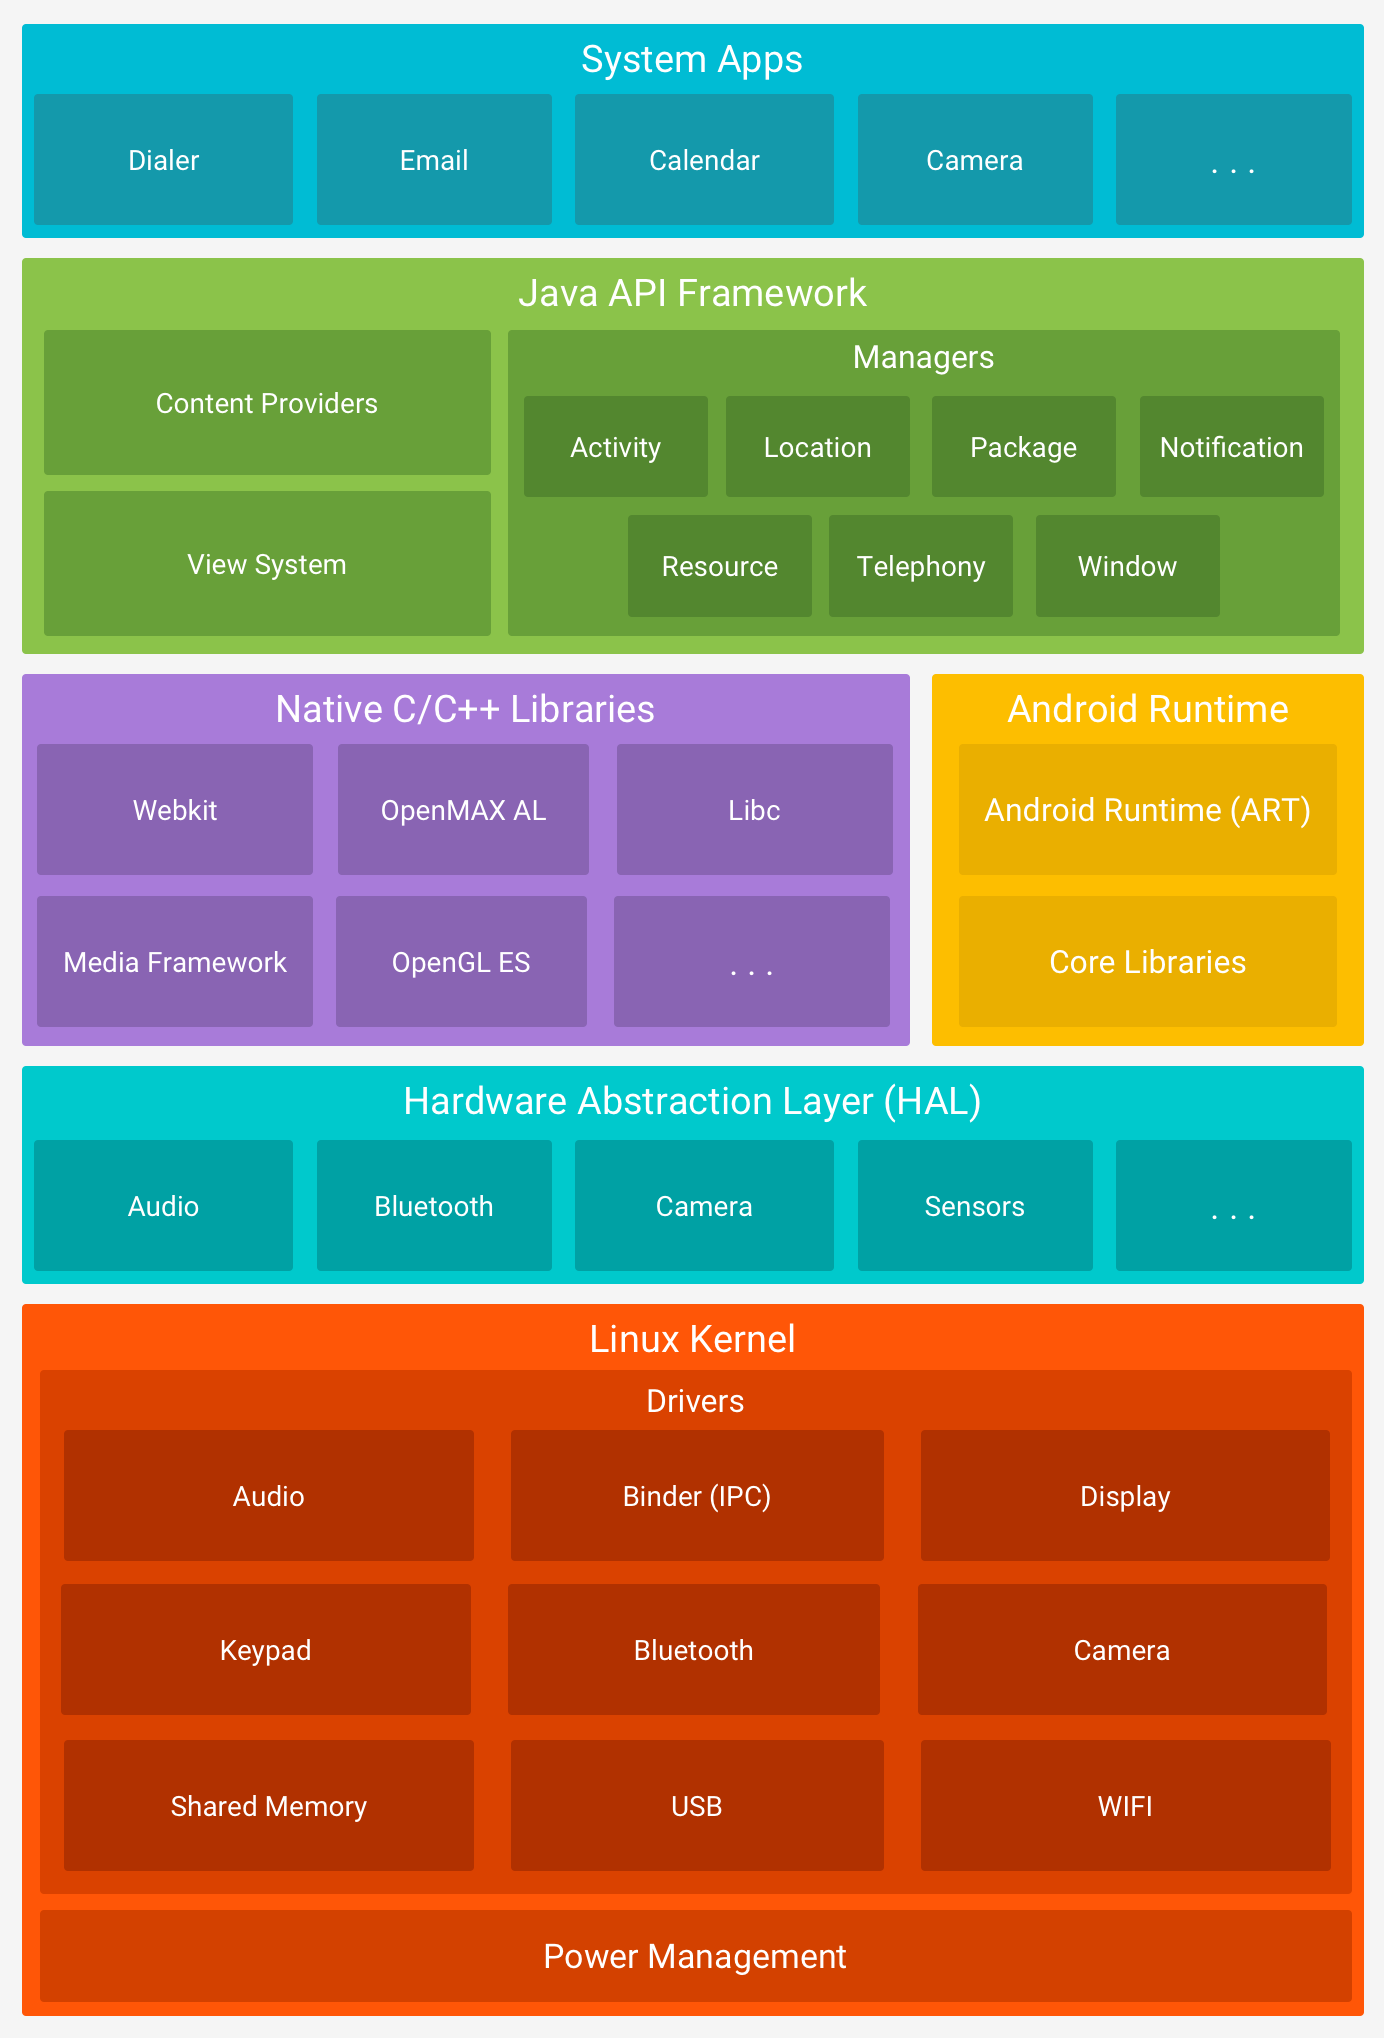
\includegraphics[width=.5\textwidth]{figures/android-stack_2x.png}
    \caption{Android 软件栈示意图}
    \label{fig:android-stack}
\end{figure}

\subsection{AOSP 分析的重要性}

在 Google 公司的主导下,AOSP 的维护行为十分频繁,对主要核心仓库的代码变动较大。根据 Google 的 Android Git repositories 中记载,仅 framework/base 仓库在 android-12.0.0\_r1 与 android-11.0.0\_r35 两个版本之间就有 151234 个提交记录,其中含有 21611 个非合并提交。其中,存在部分提交涉及数十个文件的核心代码变更。

当前活跃于市场的大多数 Android 手机的核心系统都是基于 AOSP 进一步开发。然而,在 Google 公司发布 AOSP 新版本时,各大公司均需要合入 Google AOSP 的软件变更,这为基于 AOSP 的移动系统研发部门带来了相当大的挑战。

\subsection{AOSP 分析的困难}

AOSP 作为 Android 系统的核心组成部分,是一个复杂的整体概念。对其直接展开分析是极其困难的。在对 AOSP 的整体架构进行学习之后,我主要总结出以下三点困难。这三点困难使得对 AOSP 的分析相对于其他软件项目(如 Java Web 项目、Android 应用等)更为复杂。

\begin{itemize}
    \item 独特的构建系统:Android Marshmallow 后,Google 公司选用 soong 作为 AOSP 的顶层构建系统来代替 GNU Make,并使用 ninja 作为底层构建系统加速构建过程。非泛用的构建系统为基于 AOSP 的变更分析带来了设计上的特殊性。
    \item 丰富的编程语言:AOSP 中掺杂了多种通用编程语言,包括但不限于 C,C++,Java,Kotlin,Go,Python 等。编程语言的不统一为基于源代码的分析带来了相当的复杂性。以编程语言多样性相呼应的,是项目结构的多样性。AOSP 由成千上万个不同的项目共同构成,不同的语言所使用的项目结构规范也都不相同,这使得目前许多软件分析工具无法胜任全部工作,必须针对具体情况展开具体分析。
    \item 庞大的系统架构:以 platform/framework 为例,其由 67 个仓库组成,共有 5804 个模块,而 AOSP 共拥有数千个代码仓库。与代码仓库数目众多相匹配的,是 AOSP 高度活跃的社区。在 Google 的带领下,大版本间代码变动大成为了 AOSP 的特性之一。
\end{itemize}

\subsection{系统目标简述}

本次毕业设计的题目为:“软件变更分析系统的实现”。由于 AOSP 具备上述三点分析上的困难,对其进行细致的分析工作十分艰难,因此该系统以 AOSP 下的 platform/frameworks 为例,主要围绕 “依照构建系统完成数据处理”、“变更获取”、“模块间分析” 以及 “模块内分析” 四点展开。

\begin{itemize}
    \item 在数据预处理方面,本系统希望能够获得对 AOSP 展开分析时必要的仓库模块关系以及元数据信息。
    \item 在变更获取方面,本系统希望能够使用仓库中的数据结构获得变更历史,并获得变更方法与变更类的相关信息。
    \item 在模块间分析方面,本系统希望能够根据给定遭到变更的源文件路径,获得该文件影响的所有文件路径。
    \item 在模块内分析方面,本系统希望根据变更方法,使用模块产物得到与变更方法相关的所有方法。
\end{itemize}